% \textcolor{red}{This section should present the obtained results and provide an insightful analysis of them. You can present the results using graphs, tables, or any other visualization method suits your purpose. Do not forget to include proper captions \cite{zobel2014graphs} in any of these illustration methods you use. You do not need to provide any execution details as they are already presented in Sec.~\ref{sec:experimentation}.}

% \textcolor{red}{A good practise would be to compare your algorithm with a simpler approach, such as (a) a naive method, (b) a Hill Climbing approach, or (c) a simple evolutionary algorithm. In the third case, you can use the simpler version of the algorithm you developed, i.e., the original algorithm without your modifications. In that case, you should briefly describe the comparing method(s) in Sec.~\ref{sec:experimentation}. Alternatively, you can use some reference results derived from the repositories you found some benchmark instances.}

% \textcolor{red}{To display tables, the \texttt{booktabs} package might be useful. For example, Table~\ref{tab:results_example} shows how you should increase the  size of $n$, when running your code. You can advice \cite{zobel2014graphs} to see a few examples of proper tables.}

% \begin{table}[h]
% 	\centering
% 	\caption{Example of comparison the developed algorithm's results with the best ones from a repository.}
% 	\label{tab:results_example}
% 	\begin{tabular}{lrrr}
% 		\toprule
% 		\textbf{Instance} & \textbf{Optimum (Repository xyz)} & \textbf{EA} & \textbf{time (s)} \\
% 		\midrule
% 		st70              & 678.597                           & 677.109     & 0.67              \\
% 		ei176             & 545.387                           & 544.369     & 1.16              \\
% 		kroA100           & 21285.443                         & 21285.443   & 1.69              \\
% 		rd100             & 7910.396                          & 7910.396    & 2.14              \\
% 		Pr136             & 96772                             & 96770.924   & 7.11              \\
% 		Pr144             & 58537                             & 58535.221   & 7.97              \\
% 		a280              & 2856.769                          & 2856.769    & 33.47             \\
% 		\bottomrule
% 	\end{tabular}
% \end{table}

% \textcolor{red}{You can use different illustration methods to present different aspects of your analysis. Figure~\ref{fig:plot_example} gives an example using the \href{https://www.overleaf.com/learn/latex/Pgfplots_package}{\texttt{pgfplots}} package.}

% \begin{figure}[h]
% 	\centering
% 	\begin{tikzpicture}
% 		\begin{axis}[
% 				% title={Example of convergence analysis},
% 				xlabel={Generation},
% 				ylabel={Fitness function value},
% 				xmin=0, xmax=20,
% 				ymin=290, ymax=450,
% 				xtick={0,5,10,15,20},
% 				ytick={290,300,350,400,450},
% 				legend pos=north east,
% 				ymajorgrids=true,
% 				grid style=dashed,
% 			]

% 			\addplot[
% 				color=blue,
% 				mark=square,
% 			]
% 			coordinates {
% 					(0,420)(4,411)(7,387)(10,382)(14,364)(18,360)(20,358)
% 				};
% 			\addlegendentry{EA1}

% 			\addplot[
% 				color=red,
% 				mark=triangle,
% 			]
% 			coordinates {
% 					(0,422)(4,373)(9,362)(12,312)(18,311)(20,309)
% 				};
% 			\addlegendentry{EA2}

% 			\addplot[
% 				color=violet,
% 				mark=diamond,
% 			]
% 			coordinates {
% 					(0,448)(6,401)(8,349)(11,325)(14,299)(20,298)
% 				};
% 			\addlegendentry{EA3}

% 		\end{axis}
% 	\end{tikzpicture}
% 	\caption{Example of convergence analysis.}
% 	\label{fig:plot_example}
% \end{figure}

Each genome has a score that is increased with one time unit for each person that has not arrived to their desired floor for each floor traveled by the elevator. The fitness function helps to keep track of each genome's score and gives time penalties for each person that has not arrived to their desired floor. The penalties increases the score with 100 which is a severe penalty to promote the algorithm to serve as many people as possible.

\subsection{Building 1}
As you can see in figure \ref{fig:Building1/Floors: 10, People: 10, Generation: 1000_worst} when we used our first and most primitive crossover that simply swaps the last halves of two parents genomes the best fitness value we achieved in five runs was 182. We then decided to try a new crossover that creates the first offspring with gene-by-gene selection and which parent to select a gene from is determined by a weighted random choice based on their fitness scores. The second offspring is created by reversing the first offspring.
% references here
When running the algorithm with this crossover we didn't see any improvements and the best score we achieved was also 182, see \ref{fig:Building1/Floors: 10, People: 10, Generation: 1000_best}. The first crossover reached the best value within fewer generations and seems to preform better in this instance. To be completely sure that we couldn't get improved results by changing to a different crossover without changing anything else we decided to try a much more advance crossover that had a great impact on. % references here

The third crossover uses segment-based selection instead of selecting genes individually, this method selects contiguous segments of genes from each parent. The offsets determine how many genes to take from each parent based on their fitness scores.


\begin{figure}[h]
	\centering
	\begin{subfigure}[b]{0.49\linewidth}
		\centering
		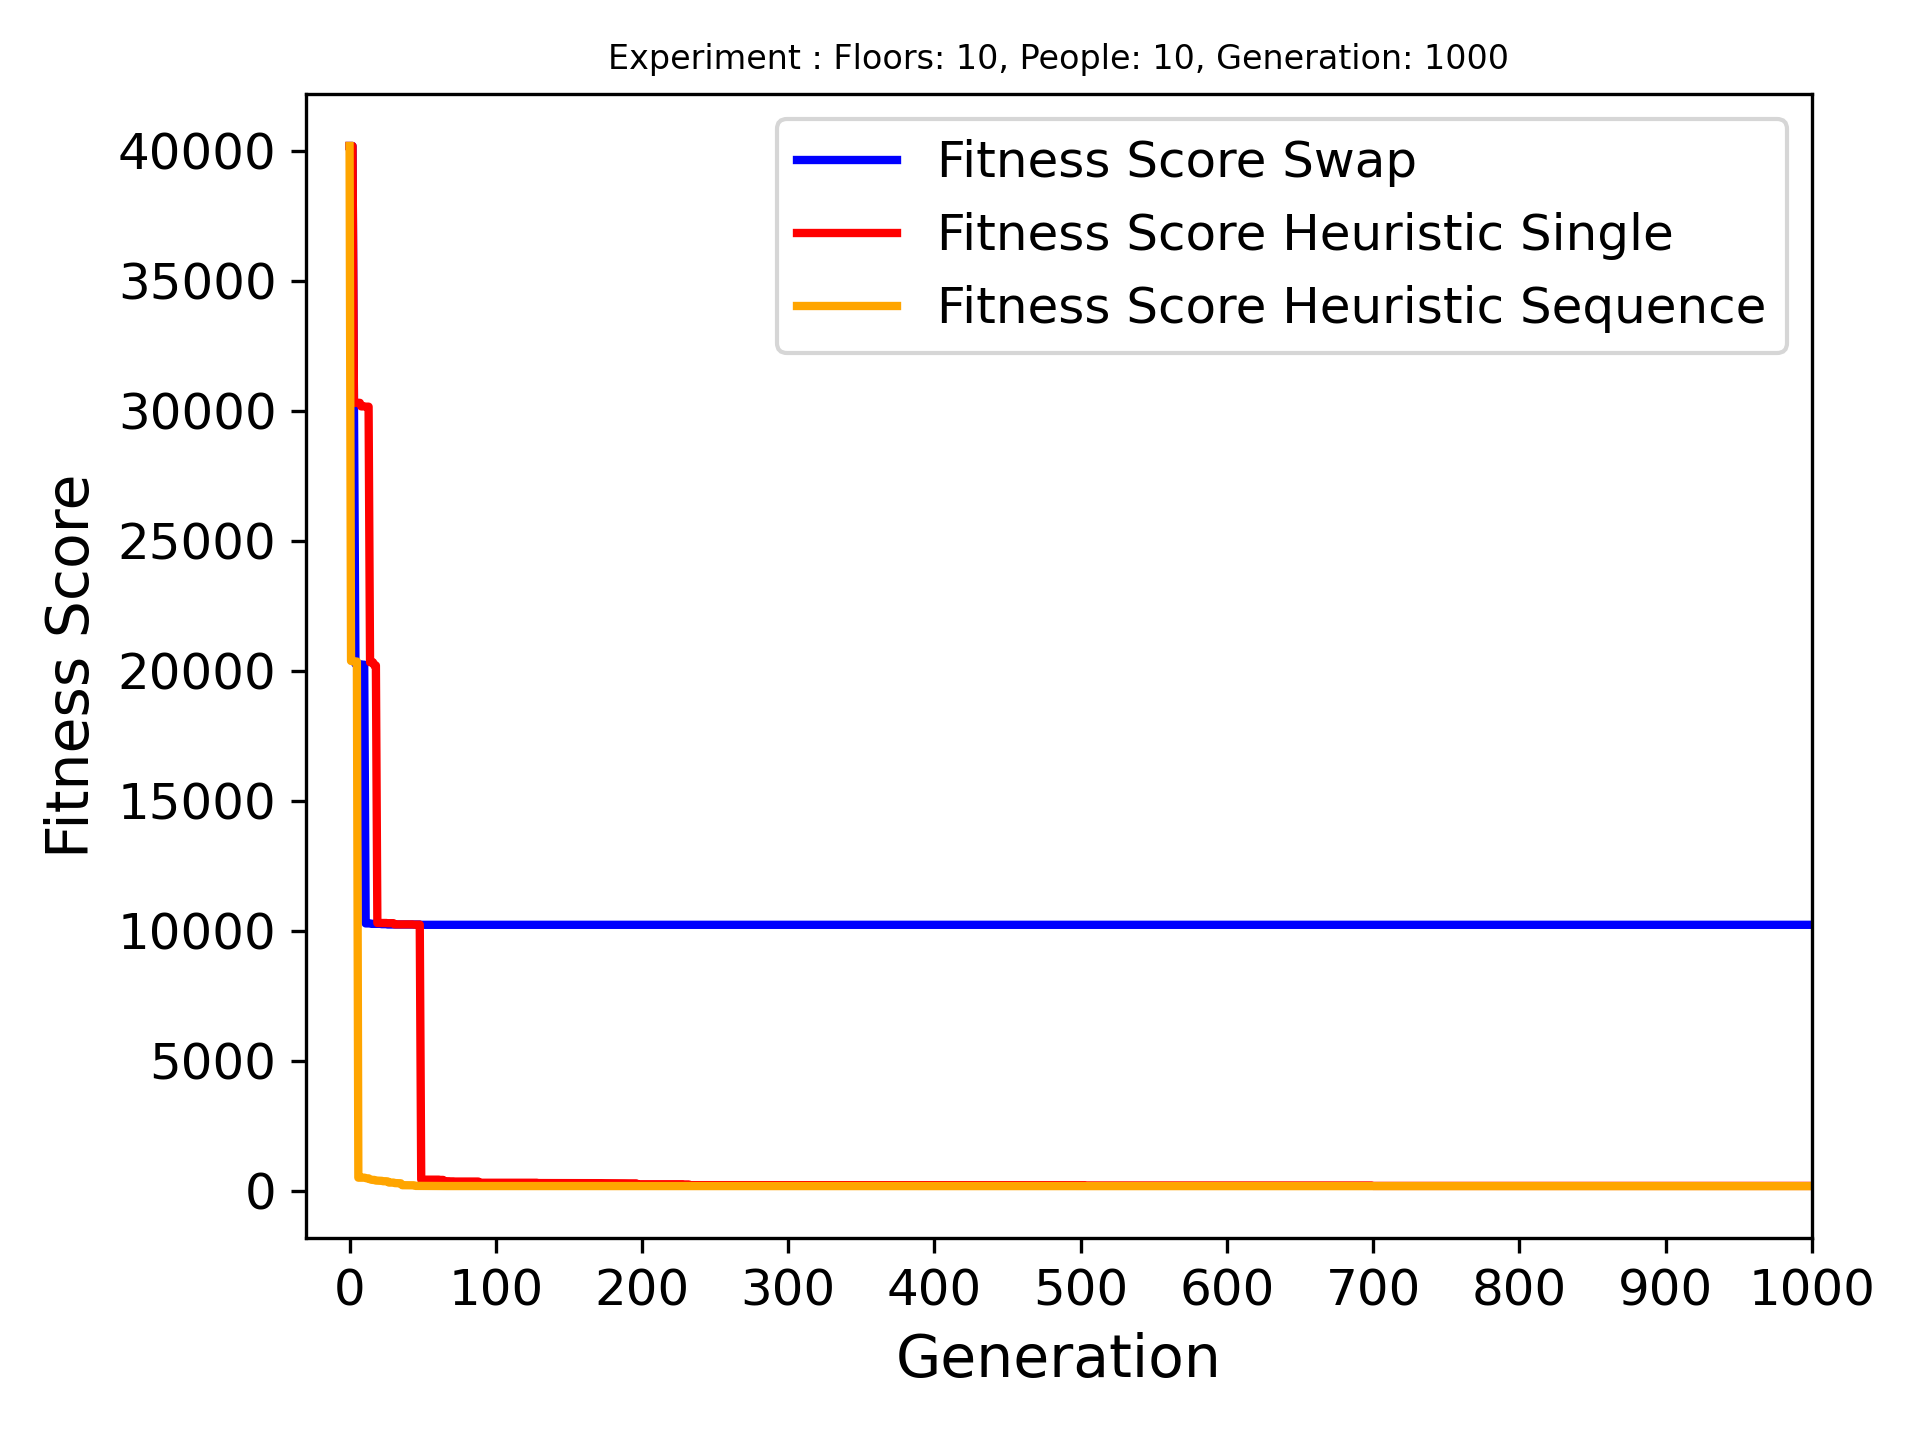
\includegraphics[width=\linewidth]{results/Building1/Floors: 10, People: 10, Generation: 1000_worst.png}
		\caption{Worst case for Building 1}
		\label{fig:Building1/Floors: 10, People: 10, Generation: 1000_worst}
	\end{subfigure}
	\hfill
	\begin{subfigure}[b]{0.49\linewidth}
		\centering
		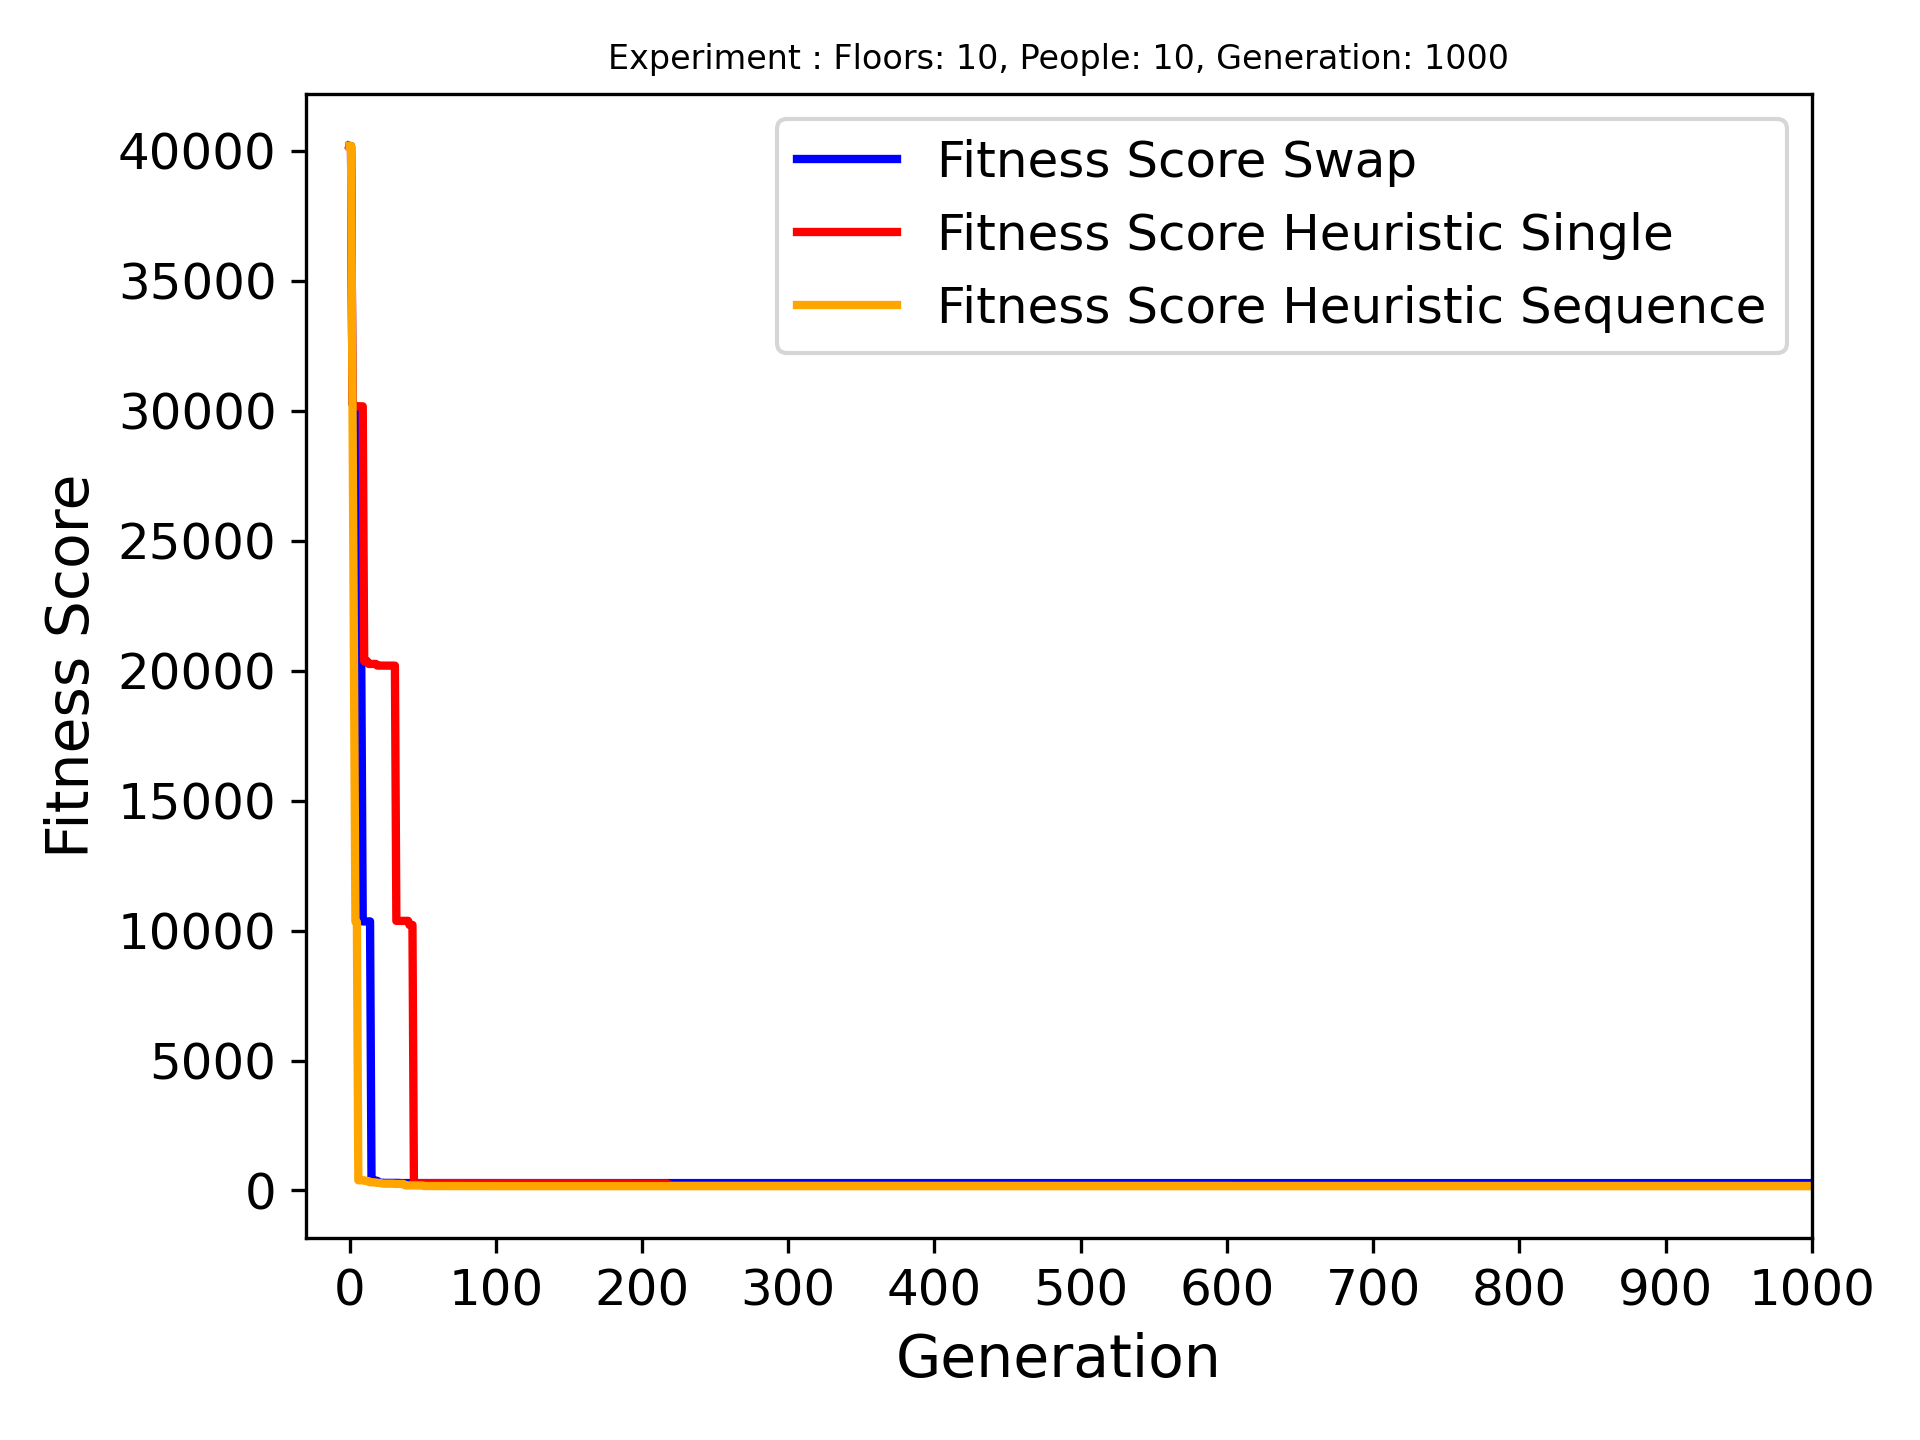
\includegraphics[width=\linewidth]{results/Building1/Floors: 10, People: 10, Generation: 1000_best.png}
		\caption{Best case for Building 1.}
		\label{fig:Building1/Floors: 10, People: 10, Generation: 1000_best}
	\end{subfigure}
	\hfill
	\label{fig:Building 1 results}
\end{figure}
\subsection{Building 3}
